\documentclass{standalone}
\usepackage{tikz}
\begin{document}
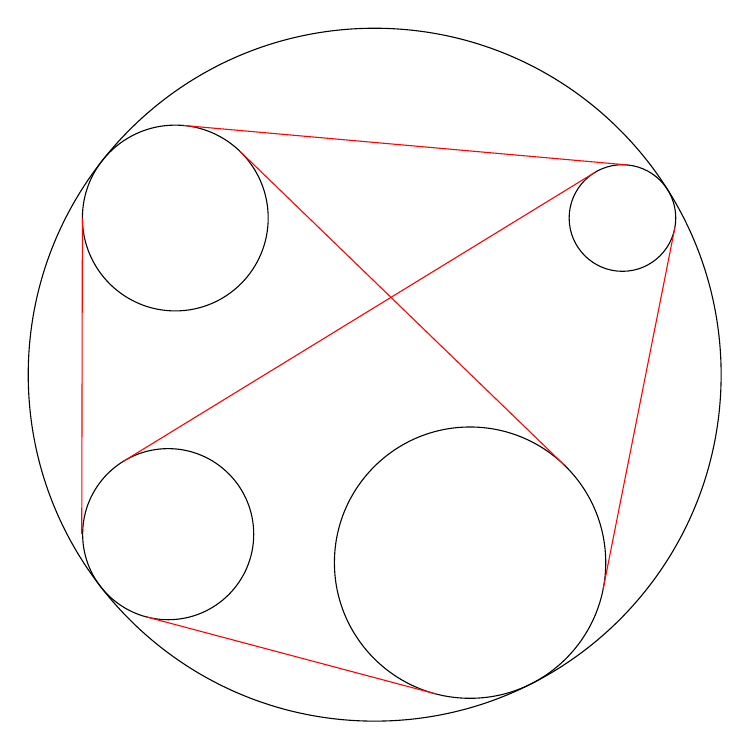
\begin{tikzpicture}[x=1pt,y=1pt]
\draw (153.35,-147.95) circle (125.19);
\draw (242.88,-91.34) circle (19.26);
\draw (81.30,-91.34) circle (33.57);
\draw (78.73,-205.58) circle (30.91);
\draw (187.82,-215.87) circle (49.02);
\draw[red] (47.73,-91.37) -- (47.50,-205.58);
\draw[red] (70.78,-235.45) -- (175.21,-263.24);
\draw[red] (104.65,-67.21) -- (221.90,-180.64);
\draw[red] (235.89,-225.42) -- (261.77,-95.09);
\draw[red] (84.28,-57.90) -- (244.58,-72.15);
\draw[red] (62.58,-179.23) -- (232.81,-74.93);
\end{tikzpicture}
\end{document}
